\documentclass[a4paper,UTF8]{article}
\usepackage[UTF8]{ctex}
%\usepackage{ctex}
\usepackage[margin=1.25in]{geometry}
\usepackage{color}
\usepackage{graphicx}
\usepackage{amssymb}
\usepackage{amsmath}
\usepackage{amsthm}
%\usepackage[thmmarks, amsmath, thref]{ntheorem}
\theoremstyle{definition}
\newtheorem*{solution}{Solution}
\newtheorem*{prove}{Proof}
\usepackage{multirow}
\usepackage{url}
\usepackage[colorlinks,urlcolor=blue]{hyperref}
\usepackage{enumerate}
\renewcommand\refname{参考文献}


%--
\begin{document}
\title{\textbf{《计算机图形学》五月报告}}
\author{161240056,谈婧,\href{mailto:jingtan@smail.nju.edu.cn}{jingtan@smail.nju.edu.cn}}
\maketitle

\section{综述}
本系统为一个包含了图形学用户界面程序和命令行界面程序的绘图系统。本绘图系统包含如下功能函数:重置画布、保存画布、设置画笔颜色、绘制线段绘制多边形、绘制椭圆、绘制曲线、对图元平移、对图元旋转、对图元缩放、对线段裁剪。

\section{算法介绍}
\subsection{DDA 数值分析}
由于线段斜率固定,所以可以通过在x或y方向上用单位1长度取样,估计另一方向增量,并对其增量和取整得到近似整数像素点。
设斜率为m,如果m<1,则从左往右在x方向上取样,每次取单位1(如果从右往左则是-1),并通过斜率计算$\delta y = m$,因此有递推式$y_{k+1}=y_k+m$。对于第k个点,$x_k = x_0 + k$, $y_k = y_0+round(k*m)$,如此就可以近似直线。如果m>1,则在y方向取样,$\delta x = \frac{1}{m}$,递推式为$x_{k+1}=x_k+\frac{1}{m}$,对于第k个点,$x_k = y_0+ round(k*\frac{1}{m})$, $y_k = y_0 + k*m$。
\subsection{Bresenham算法}
Bresenham算法引入了一个整数参量来衡量对于当前已选像素点的下一步的两个候选像素点与实际直线中下一个路径点的偏离关系,通过对于整型参数的衡量来选择下一个像素点。\\
假设在第k步确定了像素位置为$(x_k,y_k)$,那么有整型参数$p_k = \delta x(d_1-d_2) = 2\delta yx_k - 2\delta x y_k + c$($d_1$为$y_k$到y的距离,$d_2$为$y_{k+1}$到y的距离),也称为决策参数。若$p_k > 0$,即 $d_1 > d_2$,说明$y_{k+1}$比$y_k$更靠近线段,选择$(x_{k+1}, y_{k+1})$。反之$p_k < 0$,$y_k$比$y_{k+1}$更接近线段点,选择$(x_{k+1}, y_{k})$。\\
对于左端点为$(x_0,y_0)$,斜率小于1的情况:沿着x方向间隔单位1取样,在每选中像素后都计算决策参数,进行下一个像素的选择。\\
决策参数可以靠增量公式计算,$p_{k+1}-p_k = 2\delta y \cdot (x_{k+1}-x_k) - 2\delta x \cdot (y_{k+1}-y_k)$。因此如果在决策时$p_k>0$就在取高像素$(x_{k+1},y_{k+1})$的同时将决策参数的值增加$2\delta y - 2 \delta x$;如果$p_k < 0$,那么$p_k$增加$2\delta y$。\\
取样的方向和增长趋势和DDA的情况一致。
\subsection{\dots}
\dots
		
\section{系统介绍}
本系统使用python3.6开发,图形学用户界面程序由python tkinter package支持开发。本系统中的绘图核心算法在`/algorithms.py`中实现。对于每个绘图算法,除了必要的绘图所需参数传递外,增添了画布参数,方便确认需要图形绘制的特定画布。由于图形学用户界面不会和命令行界面发生交互,因此在本系统中图形学用户界面和命令行界面的实现过程中会各自自行定义画布。
\subsection{图形学用户界面设计说明}
本用户界面包含了一个App类,类在初始化时会调用每个绘图函数方法,实现各种函数调用组件,获取参数并调用algorithms.py中的核心算法绘图。
界面预览如下图:

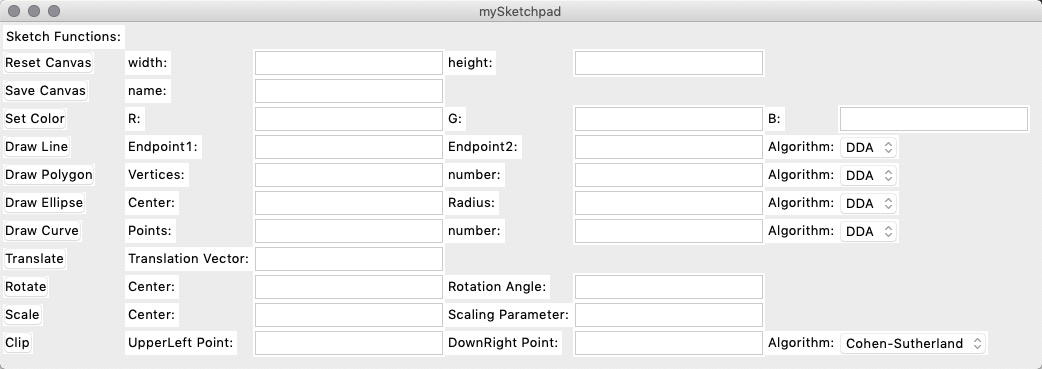
\includegraphics{picture/gui_1st.jpg}

本界面主要包含两个Tk窗口,分别为Panel和master。Panel中包含函数调用按钮,master则为绘图展示窗口。Panel的设计结构中包含一个Frame组件(PanelFrame),用于承载各种零碎部件。在PanelFrame中主要包含Button、Label和OptionMenu组件,其中Button组件用于完成算法执行按钮的设置,位置分布在最左边一栏;Label组件,用于提示系统使用步骤,提高用户友好度;OptionMenu组件用于设计绘图所需Algorithm的下拉菜单。master中主要包含一个Canvas控件,用于展现绘图结果。图形绘制时关键顶点的确定需要依靠鼠标交互,因此在设计时利用了tkinter的bind <B1-Motion> event和 <Button-1> event来确定鼠标位置和移动轨迹。用栈clickList和MotionList来保存位置变化和移动轨迹。

\section{总结}
\dots


\section{参考文献}
\bibliographystyle{plain}
	\bibliography{An Introduction to Tkinter}
	%http://effbot.org/tkinterbook/
	\bibliography{tkdocs}
	%, https://tkdocs.com/tutorial/
	\bibliography{技术博客:python – 如何让tkinter画布动态调整窗口宽度?}
	%, http://www.voidcn.com/article/p-dshhrxln-btr.html
	\bibliography{python Tkinter Programming tutorial}
	%, https://www.tutorialspoint.com/python3/python_gui_programming.htm


\end{document}